\documentclass[12pt]{exam}
\newcommand{\hwnumber}{8}
\newcommand{\hwname}{Ropes}
\newcommand{\duedate}{\formatdate{28}{03}{\YEAR} by \progDueTime}

\usepackage{../misc/latex/edition}  % Course semester
\usepackage{../misc/latex/c0}       % Listings style for c0
\usepackage{amsmath}
\usepackage{enumerate}
\usepackage[normalem]{ulem}
\usepackage{verbatim}
\usepackage[left=1in, right=1in, top=1in, bottom=1in]{geometry}
\usepackage{graphicx}
\usepackage{hyperref}
\usepackage{tikz}     \usetikzlibrary{shapes}
\usepackage{fancybox}
\usepackage[all]{xy}
\usepackage{wrapfig}
\usepackage{fancyvrb}
\usepackage{datetime}
\usepackage{etoolbox}
\usepackage{calc}
\usepackage[nomessages]{fp}
\usepackage{import}  % Like input and include, but respects subdirectories

\newcommand{\defaultQuestionLocation}{questions}
\newcommand{\inputQuestion}[2][\defaultQuestionLocation/]{%
  \subimport{#1}{#2}
}
% Subdirectories of \defaultQuestionLocation containing code and pictures
\newcommand{\code}{code}
\newcommand{\img}{img}


%%% ic: frontmatter macros
\newcommand{\specialInstructions}{}
\newcommand{\HWNUMBER}
{\ifdefempty{\hwnumber}{__}{%
  \ifnumless{\hwnumber}{10}{0\hwnumber}{\hwnumber}}}
\newcommand{\hwtype}{Written Homework}

%%% ic: 'exam' tweaks
\renewcommand{\half}{.5} % Half points

\newcommand{\Question}[2][]
 {\ifstrempty{#1}
    {\question{\bf #2}}
    {\question[#1]{\bf #2}}
  \immediate\write\rubricfile{}%
  \immediate\write\rubricfile{Question \thequestiontitle:}%
  \immediate\write\rubricfile{==========}
 }

%%% ic: Support for editable PDF
% counter name (some viewers misbehave if always the same)
\newcounter{editable}
\newcommand{\nextField}{\addtocounter{editable}{1}q\arabic{editable}}
\newcommand{\NextField}
 {\makebox[0pt][r]{\scalebox{0.1}{\color{White}\nextField}}}

% Color of edit area
\newcommand{\editAreaColor}{red}
% Single line answer:   \editableLine[extra parameters (optional)]{line width}
\newcommand{\editableLine}[2][]
{\textcolor{\editAreaColor}{%
 \underline{\hspace*{-0.25em}%
 \raisebox{-0.5ex}{%
 \TextField[width=#2, borderwidth=0, #1]{\NextField}}}}%
}
% Single line answer for code:  \editableLine[extra parameters (optional)]{line width}
\newcommand{\editableCodeLine}[2][]
{\textcolor{\editAreaColor}{%
 \underline{%
 \TextField[width=#2, height=1.5ex, borderwidth=0, #1]{\NextField}}}}
% Multiline answer:  \editableLine[extra parameters (optional)]{box height}
\newcommand{\editableBox}[2][]
{\leavevmode\hspace*{-0.1em}%
\TextField[height=#2, width=\linewidth,
           multiline=true, borderwidth=0.1, bordercolor=\editAreaColor,
           #1]{\NextField}}

%%%%% Same answer format as exams
\renewcommand{\rmdefault}{ppl}
\renewcommand{\sfdefault}{phv}
\newcommand{\answerColor}{Blue}

\ifprintanswers
\newcommand{\answer}[2]{\makebox[#1][c]{\color{\answerColor}#2}}
\else
\newcommand{\answer}[2]{\makebox[#1][c]{}\makebox[0pt]{\phantom{|}}}
\fi
\newcommand{\uanswer}[2]{\underline{\answer{#1}{#2}}}


%%% Write rubric snippet.  Usage:
% \RUBRIC
% any multi-line text (including \, #, %, whatever)
% ENDRUBRIC
%% (ENDRUBRIC should be on a line by itself)
\makeatletter
\def\RUBRIC
 {%
  \begingroup
  \let\do\@makeother\dospecials
  \endlinechar=`\^^J
  \@tofile%
 }
\def\ENDRUBRIC{ENDRUBRIC}
\def\@tofile#1^^J{%
  \def\@test{#1}%
  \ifx\@test\ENDRUBRIC
    \immediate\write\rubricfile{}  % End with an empty line
    \expandafter\@firstoftwo
  \else
    \expandafter\@secondoftwo
  \fi
  {\endgroup}%
  {\toks@{#1}%
   \begingroup\endlinechar=\m@ne
   \everyeof{\noexpand}%
   \xdef\@temp{\scantokens\expandafter{\the\toks@}}%
   \endgroup
   \immediate\write\rubricfile{\@temp}%
   \@tofile}%
}
\makeatother

%% Displays tags for an exercise in 'answer' mode
\newcommand{\TAGS}[1]
{\ifprintanswers%
  \rule{0em}{0ex}%
  \marginpar{\footnotesize%
    \fcolorbox{black}{Gray!25}{%
      \parbox[t]{2cm}{\raggedright\textbf{TAGS:}\\#1}}}%
  \ignorespaces%
 \fi}%


%% Page layout
\pagestyle{headandfoot}

\headrule
\header{\textbf{\courseNumber{} \hwtype{} \hwnumber}}
       {}
       {\textbf{Page \thepage\ of \numpages}}
\footrule
\footer{}{}{\COPYRIGHT}

\renewcommand{\partlabel}{\textbf{\thequestion.\thepartno}}
%\renewcommand{\partlabel}{\textbf{Task \thepartno}}
\renewcommand{\subpartlabel}{\textbf{\thesubpart.}}
\renewcommand{\thepartno}{\arabic{partno}}
\renewcommand{\thesubpart}{\alph{subpart}}
\pointpoints{pt}{pts}
\pointformat{\raisebox{0ex}[\height][0pt]{\fcolorbox{black}{yellow}{\themarginpoints}}}
\bonuspointformat{\raisebox{0ex}[\height][0pt]{\fcolorbox{black}{red}{\themarginpoints}}}
\marginpointname{\points}
\pointsinmargin
%\boxedpoints

\setlength\answerlinelength{2in}
\setlength\answerskip{0.3in}

\newcommand{\mkWrittenTitle}[1]{#1}
\newcommand{\mkDueDate}[1]{#1}
\newcommand{\mkEvalSummary}[1]{#1}
\newcommand{\mkGradetable}[1]{#1}



% This fixes an issue with the exam package version 2.6 and after,
% where 'framed' has been renamed to 'examframed' to avoid a conflict.
\ifcsmacro{examframed}{%
\newenvironment{framed}
{\begin{examframed}}
{\end{examframed}}
}{}

\begin{document}
\hwTitle

\noindent
For the programming portion of this week's homework, you will
implement the data structure of ropes, which provide constant-time
string concatenation.

\bigskip
\noindent
The code handout for this assignment is at
\begin{center}
\whereisthetgz{ropes-handout.tgz}
\end{center}
The file \lstinline'README.txt' in the code handout goes over the
contents of the handout and explains how to hand the assignment in.
There is a TEN (10) PENALTY-FREE HANDIN LIMIT.
Every additional handin will incur a small (5\%) penalty (even if
using a late day).

For this assignment, the last thing the autograder will do is attempt
to run your file \lstinline'rope-test.c0' against a few good data
structures and many bad ones. Putting as many test cases as you can
think of in this file will not only help you debug your code, but give
you a chance to see how your testing stacks up against a large test
suite.  (Unless you're a highly diligent tester, it's likely you'll
see many \lstinline'TEST FAILED!'  messages from this phase, but it
doesn't affect your score, only your position on the scoreboard.)

\section{Introduction to Ropes}

The most obvious implementation of a string is as an array of
characters.  However, this representation of strings --- which is also
the way that the C0 compiler implements the \lstinline'string' data
type --- is particularly inefficient at handling string
concatenation. Running \lstinline'string_join' in C0 on two strings of
size $n$ and $m$ takes time in $O(n+m)$.

A \emph{rope} is a tree-like data structure that provides a more
efficient way of concatenating strings. A rope is a pointer to a
\lstinline'rope' data structure defined in C0 as follows:
\begin{quote}
\begin{lstlisting}[numbers=none]
typedef struct rope_node rope;
struct rope_node {
  int len;
  rope* left;
  rope* right;
  string data;
};
\end{lstlisting}
\end{quote}

\clearpage
\noindent
A valid rope must be either \lstinline'NULL', a leaf, or a non-leaf.
More specifically:
\begin{itemize}
\item%
  \lstinline'NULL' is a valid rope. It represents the empty string.
\item%
  A rope is a leaf if it is non-\lstinline'NULL', has a non-empty string
  \lstinline'data' field, has \lstinline'left' and \lstinline'right' fields
  that are both \lstinline'NULL', and has a strictly positive \lstinline'len'
  equal to the length of the string in the \lstinline'data' field (according
  to the C0 string library function \lstinline'string_length').
\item%
  A rope is a non-leaf if it has non-\lstinline'NULL' \lstinline'left'
  \emph{and} \lstinline'right' fields, both of which are valid ropes, and if
  it has a \lstinline'len' field equal to the sum of the \lstinline'len'
  fields of its children. The \lstinline'data' field of a non-leaf is
  unspecified.  We'll call these non-leaves \emph{concatenation nodes}.
\end{itemize}

This is one of many ropes that represents the 15-character string
\lstinline'"happy birthday!"':
\begin{center}
  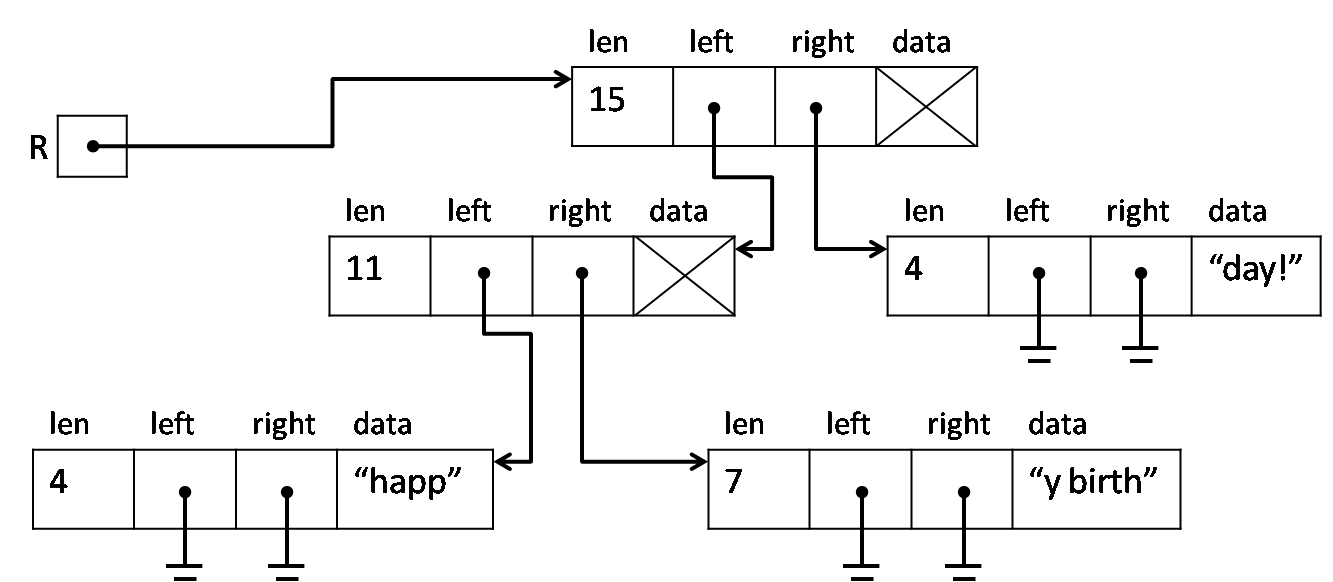
\includegraphics[width=.85\textwidth]{img/rope-concrete.png}
\end{center}
Note that where we indicate Xes in the \lstinline'data' field, any contents
would be allowed and we would still have a valid rope. We can also represent
the same structure using a short-hand notation that illustrates the
two different types of nodes, leaf nodes and concatenation nodes:
\begin{center}
  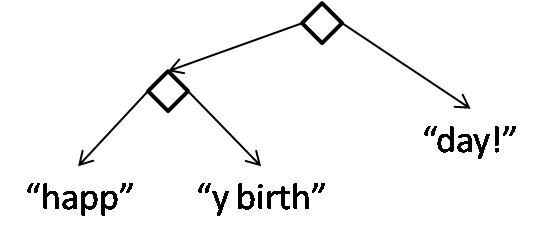
\includegraphics[width=.35\textwidth]{img/rope-abstract.png}
\end{center}

\begin{task}[4]
\TAGS{ds-invariant, pointer, string}
In the file \lstinline'rope.c1', write a data structure invariant
\lstinline'bool is_rope(rope* R)'. For full credit, you should ensure
that your data structure invariant terminates on \underline{all}
inputs.  HINT: If your circularity check requires more than 2-6 extra
lines, you're doing it wrong.
\end{task}

\section{Implementing Ropes}

A full interface for ropes would presumably need to mimic the entire
C0 string library. In this section, we'll just be implementing a
limited subset of this library.

\begin{quote}
\begin{lstlisting}[numbers=none]
// typedef _______* rope_t;
int rope_length(rope_t R)
  /*@ensures \result >= 0; @*/ ;
rope_t rope_join(rope_t R, rope_t S)
  /*@requires rope_length(R) <= int_max() - rope_length(S); @*/ ;
char rope_charat(rope_t R, int i)
  /*@requires 0 <= i && i < rope_length(R); @*/ ;
rope_t rope_sub(rope_t R, int lo, int hi)
  /*@requires 0 <= lo && lo <= hi && hi <= rope_length(R); @*/ ;
\end{lstlisting}
\end{quote}
Functionally, these four functions should do the same thing
as the similarly-named function in the C0 \lstinline'string' library.
We'll also implement two functions for converting between C0 strings
and our data type of ropes.
\begin{quote}
\begin{lstlisting}[numbers=none]
rope_t rope_new(string s);
string rope_tostring(rope_t R);
\end{lstlisting}
\end{quote}


When we talk about the big-$O$ behavior of rope operations, we assume
for simplicity the rope's leaves contain strings that are smaller than
some small constant, which means that all operations on C0 strings can be
treated as constant-time operations.

\begin{task}[5] \textbf{Constant time operations.}
\TAGS{ds-invariant, pointer}

\noindent
In the file \lstinline'rope.c1', implement the $O(1)$ functions
\lstinline'rope_new', \lstinline'rope_length', and \lstinline'rope_join'.
\end{task}

The \lstinline'rope_new' function takes any C0 string and returns a rope without
any concatenation nodes. The \lstinline'rope_join' function is able to
work in constant time
because, at most, it has to allocate a single concatenation
node:
\begin{center}
  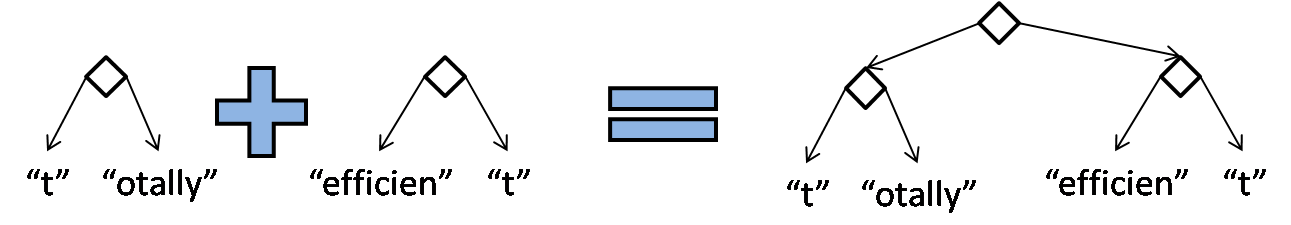
\includegraphics[width=.85\textwidth]{img/rope-join.png}
\end{center}

In the example above, the client of the rope library
can continue using the rope representing \lstinline'"totally"' even
though the allocated memory for that rope is a part of the rope
representing \lstinline'"totallyefficient"'. This \emph{structure sharing}
between different ropes means that, while ropes are a data structure
that we can treat like a tree, the memory representation may not
actually be a tree.
Here's another example: if \lstinline'R1' is rope for
\lstinline'"totally"' above and \lstinline'R2' is the rope for
\lstinline'"efficient"' above, then executing the expression
\lstinline'rope_join(rope_join(R1, R2), rope_join(rope_new(", "), R1))'
will produce the following structure in memory:
\begin{center}
  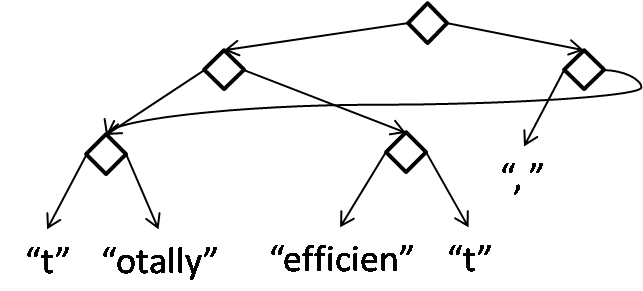
\includegraphics[width=.43\textwidth]{img/rope-join2.png}
\end{center}
Structure sharing for ropes only works because none of the rope
interface functions allow us to modify ropes after they have been
created. By sharing structure, we can make very very big strings
without allocating much memory, and this is one reason it was necessary
to add the precondition checking for overflow to \lstinline'rope_join'.

\begin{task}[4] \textbf{Simple recursive operations.}
\TAGS{ds-invariant, pointer, string}

\noindent
In the file \lstinline'rope.c1', implement the recursive functions
\lstinline'rope_charat' and \lstinline'rope_tostring'.
\end{task}

\bigskip
Your implementation of \lstinline'rope_charat' should take, in the worst
case, time proportional to the \emph{height} of the rope. If we kept
ropes balanced, this would mean that \lstinline'rope_charat' would take
time in $O(\log n)$, where $n$ is the length of the rope as reported
by \lstinline'rope_length'. We will not, however, implement balancing in
this assignment, and none of the code you write in this section should
modify the structure of existing ropes in any way.

The \lstinline'rope_tostring' function returns the string that a rope
represents.  There's a way to implement this function so that its
running time is in $O(n)$, but this would be overkill.  Just implement
the most natural recursive solution possible, which uses
\lstinline'string_join'.

\bigskip

Sharing between ropes gets more interesting once we start considering
the \lstinline'rope_sub' function. The C0 library function
\lstinline'string_sub(s,lo,hi)' returns the segment of the string \lstinline's'
from index \lstinline'lo' (inclusive) to index \lstinline'hi' (exclusive). The
function \lstinline'rope_sub' must do the same thing, without changing the
structure of the original rope in any way, while also maximizing
sharing between the old rope and the new rope and only allocating a new
node when it is impossible to use the entire string represented by an
existing rope.

\clearpage
Here are some examples, where we have \lstinline'R' as the rope representing
\lstinline'"totallyefficient"' from the previous page.

\medskip\noindent
After running \lstinline'rope_t R3 = rope_sub(R, 1, 16);'
\begin{center}
  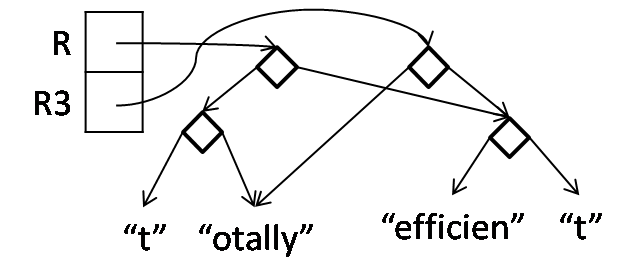
\includegraphics[width=.4\textwidth]{img/rope-sub1.png}
\end{center}

\medskip\noindent
After running \lstinline'rope_t R3 = rope_sub(R, 1, 11);'
\begin{center}
  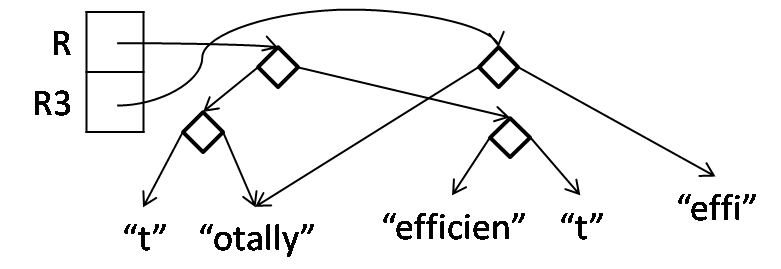
\includegraphics[width=.48\textwidth]{img/rope-sub2.png}
\end{center}

\medskip\noindent
After running \lstinline'rope_t R3 = rope_sub(R, 2, 11);'
\begin{center}
  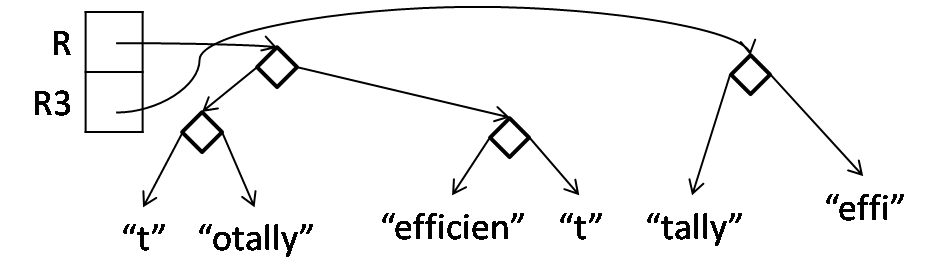
\includegraphics[width=.55\textwidth]{img/rope-sub3.png}
\end{center}


Running \lstinline'rope_sub(R,0,1)' and \lstinline'rope_sub(R,7,16)' should not
cause \emph{any} new memory to be allocated, because these
substrings are captured by subtrees of the original rope. Running
\lstinline'rope_sub(R,2,3)' must return a newly-allocated leaf node
containing the string \lstinline'"t"'. % When doing
%\lstinline'rope_sub(R,lo,hi)', in other words, we
% expect you to do structure sharing only for the subropes that fall in
% the range from \lstinline'lo' (inclusive) to \lstinline'hi' (exclusive).

\begin{task}[7]
\TAGS{ds-invariant, pointer, string}
In the file \lstinline'rope.c1', implement the recursive function
\lstinline'rope_sub'. Without changing the structure of the original
rope in any way, this function should minimize memory allocation
by sharing as much of the original rope as possible.
\end{task}

\bigskip
\noindent
HINT: in your recursive function, try to first identify all the cases where it
is possible to return immediately without any new allocation. What cases are
left?

\clearpage
\section{Reducing Memory Usage}

The \lstinline'rope_join' and \lstinline'rope_sub' functions use sharing to
reduce memory usage, but we specified that they should not change the
structure of existing ropes. For this task, you will write a
memory-reduction procedure that changes the structure of existing
ropes to conserve memory without changing the strings that those ropes
represent.
\begin{center}
  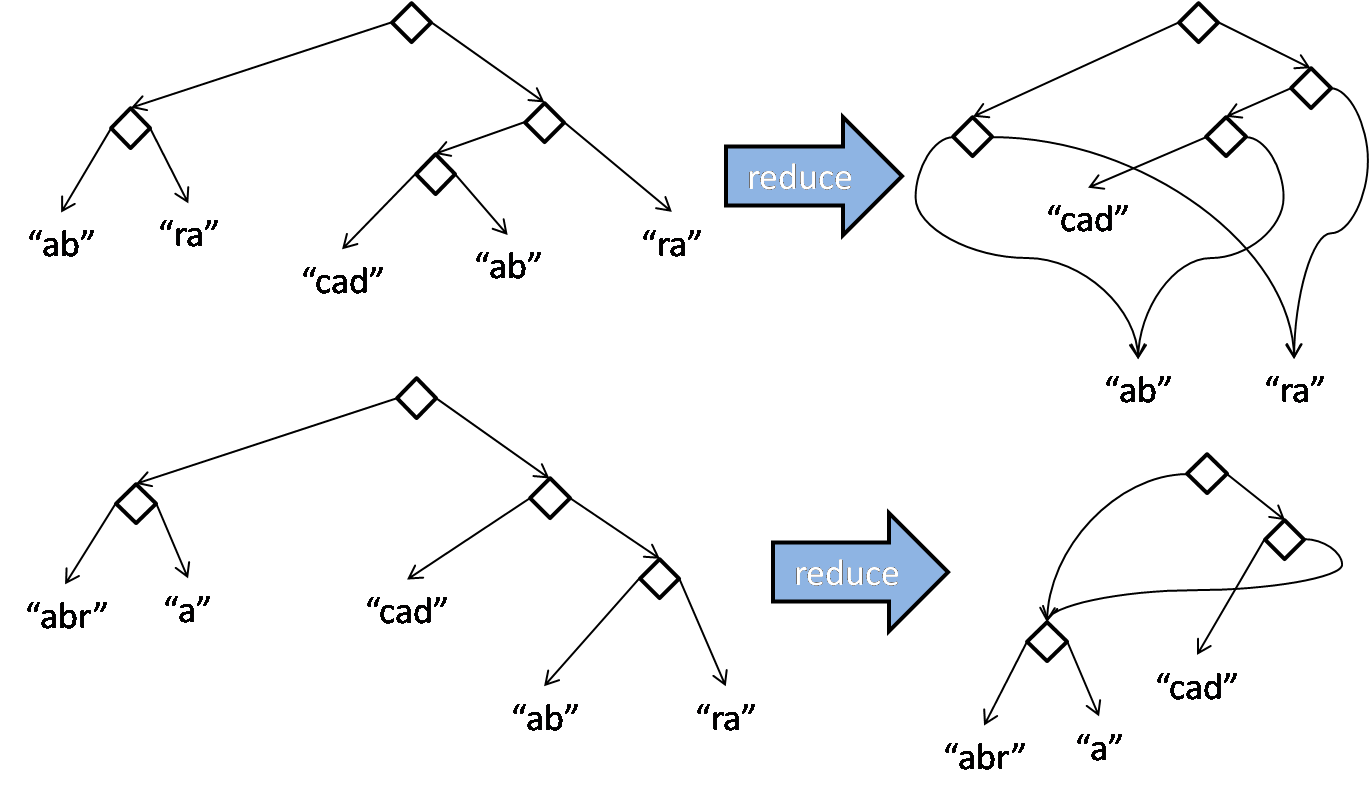
\includegraphics[width=.8\textwidth]{img/reduce.png}
\end{center}

Your memory-reduction procedure will use a hashtable-based
dictionary. When given a rope, you should look up that rope in the
dictionary to see if an equivalent rope (one representing the same
string) already exists. If so, your memory-reduction procedure can
just return that already-stored rope in place of the rope you were
given.

If your memory-reduction procedure doesn't find the rope already in
the dictionary, it should recursively call itself, first on the left
sub-rope, and then on the right sub-rope. Then, without allocating any
additional memory, you can replace the original left and right
sub-ropes with the results of calling the memory-reduction procedure
on them. (It's always okay to replace a rope with another rope that
represents the same string.) Now you have a rope with two
sharing-maximized sub-ropes; this new rope should be added to the
dictionary for future use.

\begin{task}[5]
\TAGS{dictionary, hashing, function-pointer, pointer}
  In the file \lstinline'rope.c1', implement the function
  \lstinline'rope_reduce' using a helper function. This function takes
  an array \lstinline'A' of ropes, allocates a dictionary, and runs
  the memory-reduction procedure on each of the ropes in the
  array. Ropes and sub-ropes stored in lower indices should remain in
  the dictionary and be re-used when processing ropes and sub-ropes
  stored in higher indices.
\end{task}

More examples of what \lstinline'rope_reduce' does can be found on the next
page.  You'll need to write functions to initialize the client
interface of generic hashtable-based dictionaries. The simplest way to
write the \lstinline'key_hash_fn' and \lstinline'key_equiv_fn' functions
involves repeatedly using \lstinline'rope_charat'. That implementation will
work fine for this assignment, but it is possible to create a more
efficient version.

\clearpage

\noindent
More examples of how we expect \lstinline'rope_reduce' to work:
\begin{center}
  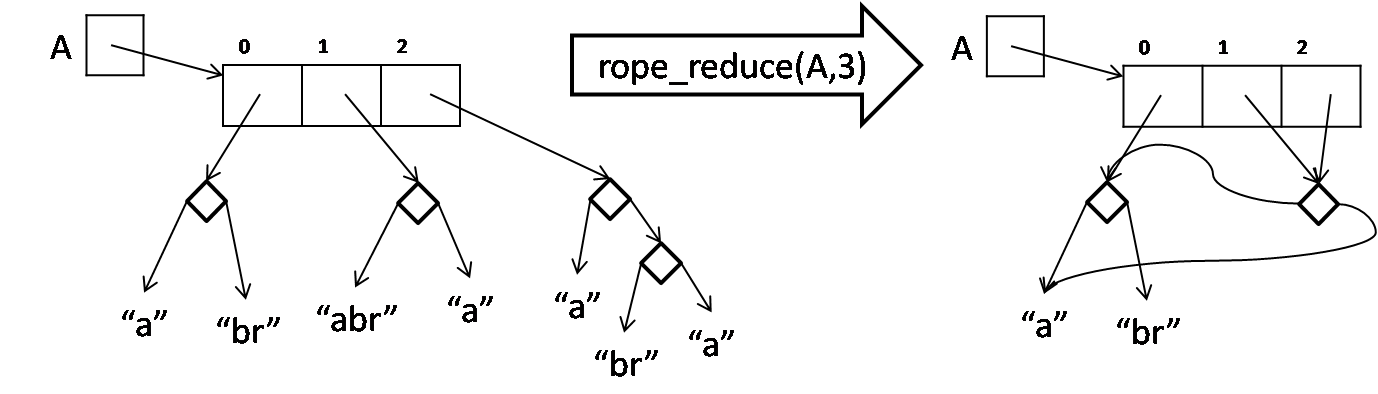
\includegraphics[width=.9\textwidth]{img/rope-reduce1.png}
\end{center}
\begin{center}
  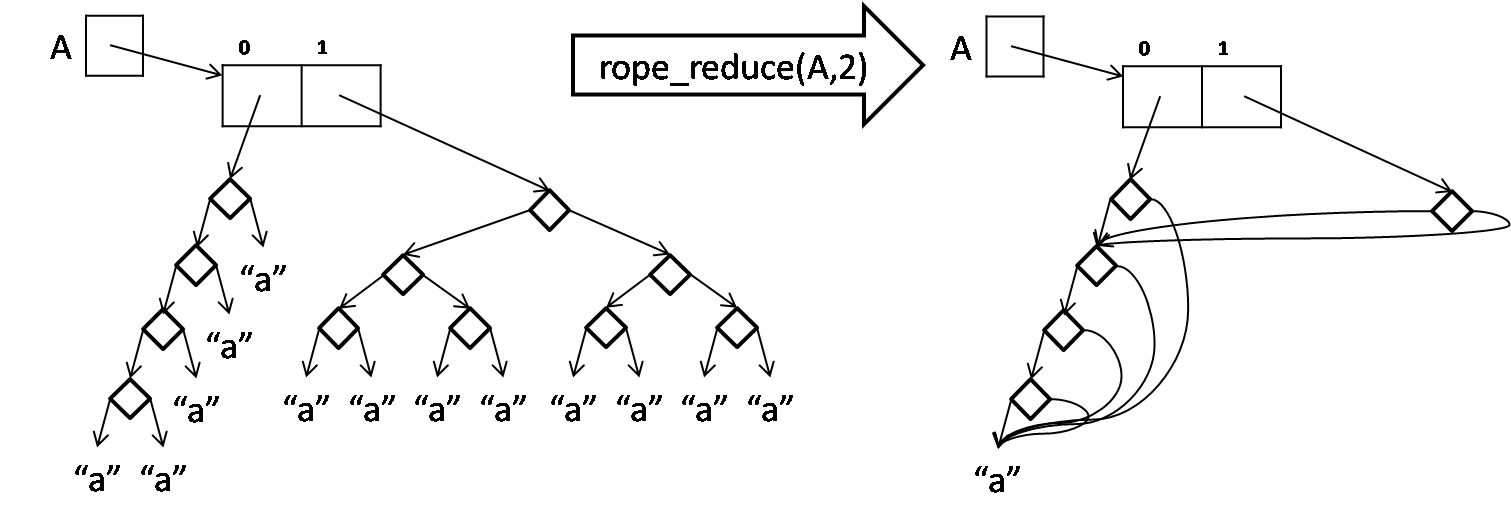
\includegraphics[width=\textwidth]{img/rope-reduce2.png}
\end{center}
\begin{center}
  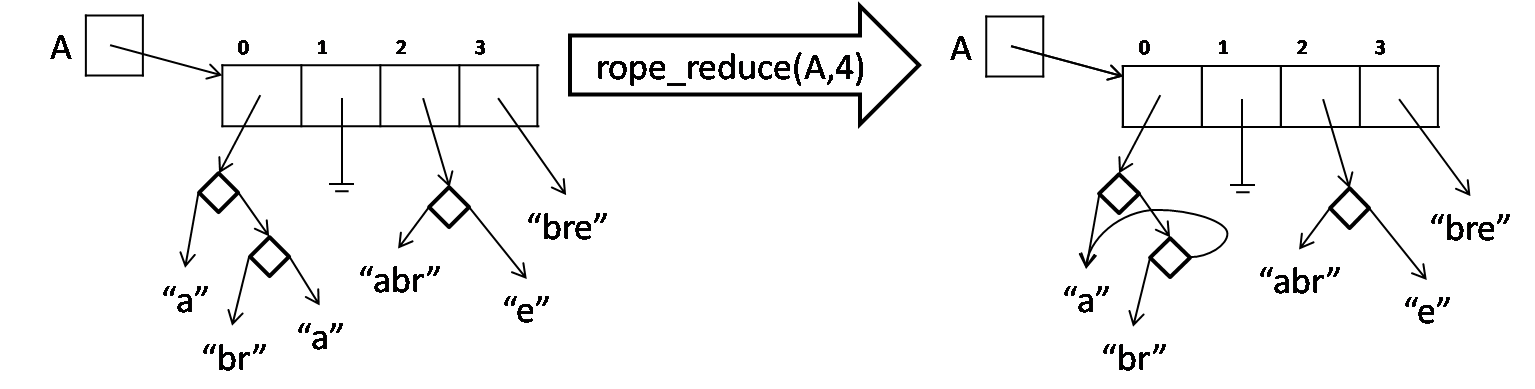
\includegraphics[width=\textwidth]{img/rope-reduce3.png}
\end{center}


\end{document}
